\chapter{<Theoretical Background>}
% \thispagestyle{fancy}
In this chapter, a detailed description about background of the degree project is presented together with related work. Discuss what is found useful and what is less useful. Use valid arguments.

Explain what and how prior work / prior research will be applied on or used in the degree project /work (described in this thesis). Explain why and what is not used in the degree project and give valid reasons for rejecting the work/research.

Use references!

\section{Use headings to break the text}
Do not use subtitles after each other without text in between the sections.

\section{Related Work}

Spiking neural networks for control have been used in many different contexts, e.g for robotic movement, digit recognition\cite{lee_training_2016} or object detection\cite{soures_deep_2019}\cite{zhou_deep_2020}.\\
In \cite{bouganis_training_2010} spiking neurons are used to control target reaching movements of a 4-DoF robotic arm using a plausible neuron model and learning rule. In their approach they lean into the DIRECT model of \cite{bullock_self-organizing_1993}, which learns the a priori unknown robot kinematics by randomly repeating movement commands and learning the resulting translation of the end effector.\\
Another approach for robotic arm control comes from \cite{dewolf_spiking_2016} using the \ac{NEF}\cite{eliasmith_neural_2004}, in which different regions of the brain have been simulated to generate the trajectory as well as the control signals.\todo{Is this to general?}\\
The authors of \cite{bing_supervised_2019} summarized several approaches for robotic control of flying or driving robots and used layered spiking neurons with a local learning rule to train the network to reach the target while avoiding obstacles.\\
While each of these models inherit some biologic plausibility, they only take one or a few aspects of biological plausibility into their model, be it the neuron model, the learning rule, encoding or network structure. Furthermore are these approaches often targeted towards the application of robotic arm and not general control of dynamic systems.\\
Spiking neurons have also been used for PID controllers. In \cite{lu_spiking_2011} it is shown that a PID controller is possible using three neurons, one for P,I and D respectively. However no example using the network as an example is shown. Furthermore the learning is based on individual parameter tuning for each neuron. Lastly the robustness of 3 neurons is not biologically plausible.\\
In \cite{stagsted_towards_2020} a PID controller is designed using spiking neurons on neuromorphic hardware in order to control a 1-DoF UAE.\\
However it is unclear how the network was trained on the neuromorphic hardware or how this approach can be adapted to bigger systems.\\


TODO &&&&
start looking at the F.Zenke stuff\\
Check the review papers that are open



This one only learn the kinematics and not any dynamic system.\\

Name prewitten libs for neural simulation
brian nengo NeMo norse snntorch spinnaker
bindsnet \& snntorch based on pytorch

You should probably keep a heading about the related work here even though the entire chapter basically only contains related work.

Here just what has been done for each of the headlines\\
Previous efforts were already made to control dynamic systems with \acp{SNN}.
\todi{List here also efforts with other concepts apart from Balanced Networks}




Neural networks in general
spiking neural networks and their differences and what they are better for.
neuron models, iwazishi neuron and maybe one more
mein neuron model und warum ich es ausgewaelt habe: einfach zu implementieren. Bereits fuer dynamische systeme verwendet,
Nachteile dieses modells.
Vlt vergleich mit einem anderen modell.
Ganz kurzer ausflug in die regelung von dynamischen systemen.


What is a neural network? -> not here ref a paper. kurze erkl'rung in der einfuerung
in der einfuhurng vlt auch hodgekin huxley erwaehen :)




\section{Autoencoder}
An autoencoder is a type of neural network for learning a representation of its input. It consists of an encoder and decoder function $z =f(x)$ \& $\hat{x} = g(z)$. The encoder function from the input space, e.g $\mathbb{R}^n$, to a encoded space $\mathcal{C}$. The decoder is then decoding the data from $\mathcal{Z}$ back to $\mathbb{R}^n$. The goal is that the representation is as accurate as possible. This is easy in case the if $\mathcal{Z}$ is equal or larger than the input space. Then every possible input can be encoded by its own value as
\begin{equation}
\begin{aligned}
 	z = f(x) &= x\\
 	\hat{x} = g(z) &= z = x
\end{aligned}
\end{equation}
which is not useful. $\mathcal{Z}$ has to many DOF and can "memorize" each input. In most cases however $\mathcal{Z}$ is constrained that the autoencoder has to find the relevant properties of the input. This is often done by reducing the dimension if $\mathcal{Z}$ or by regularization. Regularization is added to the Loss
\begin{equation}
	L(x,\hat{x}) + C(z)
\end{equation}
where L can be e.g. MSE and the regularization term $C$ can enforce sparsity or other properties\cite{goodfellow_deep_2016}.


\section{Neuron model}

\subsection{Biological Neuron model}
The first biologically accurate model of neuron spiking behaviour is the \ac{HH} model from 1952\cite{hodgkin_currents_1952}. Since then the \ac{HH} model has been extended in multiple ways to cover more e.g. different ion channels. The \ac{HH}-model considers the neuron with its ion channels. The membrane acts as a capacitance and the travelling ions in each ion channel contribute a current to the overall membrane potential. These ion gates are voltage dependent and are defined positive in direction out of the cell.\\
A particular ion channel for ion $X$ can be modelled as
\begin{equation}
	I_X= g_X \cdot (V-V_X)
\end{equation}
These currents are summed summed for the different ion channels in question, most commonly for Sodium, Potassium and a leak current. In reality there are a plethora of different channels and channel properties\footnote{See  \url{channelpedia.epfl.ch} for an extensive list}. The $V_X$ are the equilibrium potentials for each of the channels and can be computed using the Nernst equation \cite{johnston_foundations_1995}.
\begin{equation}
	C \frac{dV}{dt} = g_{Na} \cdot (V-V_{Na}) + g_K \cdot (V-V_K) + g_l \cdot (V-V_l)
\end{equation}
Do model the voltage dependency of the ion channels, the conductances are described with gating variables, usually called $n$, $h$ and $g$ for Na-Activation, Na-Inactivation and K-activation respectively. One gating variable is set between $[0,1]$ and models the permeability of said gate. Multiple gates are used to fit to each ion channel in order to match experimental data and the model behaviour.\\
Gates have first order dynamics of the form
\begin{equation}
	\frac{dn}{dt} = \alpha_n(1-n) - \beta_n n
\end{equation}
for e.g the n gate. The other gates' dynamics are analogous. The functions $\alpha$ and $\beta$ are voltage but not time dependent. The discussion of initial values as well as functions for $\alpha_p,\ \beta_p\ \ p = (n,h,m)$ can be found in \cite{hodgkin_quantitative_1952} or \cite{johnston_foundations_1995}. The gates for each ion channel's conductance are found to be
\begin{equation}
	\begin{aligned}
	g_{Na} &= \bar{g}_{Na} n^4\\
	g_{K} &= \bar{g}_{K} m^3h\\
	\end{aligned}
\end{equation}
and give form to the final model
\begin{equation}\label{eq:HH}
	\begin{aligned}
	C\frac{dV}{dt} &= I(t) -\bar{g}_{Na} n^4(V-V_{Na}) - \bar{g}_{K} m^3h(V-V_{K}) -g_L(V-V_{L})\\
	\frac{dn}{dt} &= (1-n)\alpha_n(V) - \beta_n n (V)\\
	\frac{dm}{dt} &= (1-m)\alpha_m(V) - \beta_m m (V)\\
	\frac{dh}{dt} &= (1-h)\alpha_h(V) - \beta_h h (V)
	\end{aligned}
\end{equation}
We did not define a gate for the leak term as it is assumed constant.
\subsection{"IF and LIF"}
In contrast of the \ac{HH} model in \cref{eq:HH}, the simplest models of neurons are the \ac{IF} and \ac{LIF} models.\\
\paragraph{IF Neurons}
\ac{IF} Neurons, as the name implies, integrate the incoming current over time.
\begin{equation}
	\frac{d V(t)}{d t} = \frac{1}{C}I(t)
\end{equation}
The membrane voltage is governed by the incoming current spikes of connected neurons and the membrane capacitance. The neuron potential does not change without a change of input current and thus presents as a perfect integrator of the input.\\
\paragraph{\ac{LIF} Neurons}
In contrast to that the \ac{LIF} neuron contains a leak term on the RHS which brings the voltage back to its resting potential over time. The model can be expressed as
\begin{equation}
	\tau\frac{dV(t)}{dt} = -(V(t)-E_r) + RI(t),
\end{equation}
where $\tau = RC$ is the time constant the composed of the membrane resistance $R$ and the membrane capacitance $C$ and the resting potential $E_r$. In the absence of input $I(t)$ the voltage settles on the membrane potential $E_r$.\\
The input $I(t)$ encapsulates external inputs as well as a sum of Dirac functions indicating a spiking neuron
\begin{equation}
	I(t) = \sum_k \delta(t-t^k)
\end{equation}
\rewrite{This is not truly correct. Forgot weights, but at the same time only when there are more than 1 neuron}
and $t_k$ being the time of the $k$-th spike. When the membrane voltage exceeds the threshold potential $\bar{v}$, a spike is sent out by the neuron and the voltage sets back to its reset voltage $v_{res}$.
\subsection{Izhikevich Neuron}
While the above models deliver a useful and cheap simplification, they lack in accuracy. The Izhikevich model \cite{izhikevich_simple_2003} of the neuron tries be the of both worlds in terms of efficiency and accuracy. It is comprised of 2D ODEs with the membrane potential $v$ as
\begin{equation}
	\begin{aligned}
	\frac{d v}{dt} &= 0.04v^2 + 5v + 140 -u +I(t)\\
	\frac{d u}{dt} &= a(bv-u).
	\end{aligned}
\end{equation}
With the chosen factors, the neuron experiences a spike when $u\geq30 $mV, in which case the neuron resets to
\begin{equation}
\begin{aligned}
	u &\leftarrow u+d\\
	v&\leftarrow c
\end{aligned}
\end{equation}
The parameters describe $a$ scale of recovery, $b$ sensitivity, $c$ the reset potential of $v$ and $d$ the reset of variable $u$.\rewrite{Maybe shitty explanation, which could be extended on.} Depending on these parameters one can achieve different behaviours of the neuron e.g. regular spiking, fast spiking and low threshold spiking to name a few \cite{izhikevich_simple_2003}.



\subsection{Synaptic intelligence}
In addition to the neuron model




\section{Neural Networks}

\subsection{Artificial Neural Networks}
 \todo{Make clear distinction between forward nns and ann. Bcs apparently they are not the same!}


Copying nature to solve engineering problems is not a novel practise and also for neural networks this is not new. Many different network architectures with different levels of biologic plausibility have been investigated and published and there is no consent in the design decisions. As a result different choices are made by different researches leading to various approaches that are similar and yet different. Biologic realness can be chosen on different parts of the network. Therefore it is impossible to inspect each nuisance explicitly. Apart from very specific implementations we illustrate below many \acp{SNN} can be categorized in different segments of which we highlight certain designs seen in the literature.\\

\subsubsection{Neuron model}
	As outlined above the neuron model can have different complexities and accuracy. By far the most used model in the literature are \ac{LIF} and \ac{IF} model.
\subsubsection{Encoding}
	The coding of information plays a crucial role it a \ac{SNN}. Since the network is working on discrete spikes, a methodology needs to be implemented to convert e.g continuous values in spikes. To let the network be susceptible to the outer world, a subset of neurons of the network are exposed to these external inputs.\\
	\paragraph{\ac{TTFS}}
	In this coding scheme the information of an input is solely encoded in the time between the external input and the time neurons fire a spike. A simple visualization could be by implementing the stronger the input the sooner the input neuron spikes after the input onset.\\
	An extension of this idea is rank order coding, where the ordering of spikes encodes information\cite{thorpe_spike-based_2001}.\\
	\paragraph{Phase coding}
	Phase coding is a slight variation of the \ac{TTFS} code. In certain areas of the brain show oscillations similar to a clock\cite{jacobs_critical_2013}. The premise of phase coding is that the oscillation of this clock can be used to convey information. Thus, a spike relative to the phase of a clock cycle entails information on the input signal.\\
	\paragraph{Rate coding}
	Rate coding transforms the intensity of a signal to a spiking pattern with a corresponding frequency. The intensity is often normalized to realistic spiking frequencies. Since the brain is noisy, the spike is not fired with the respective rat but rather with a Poisson process given suitable rate $\lambda$.
	Using a Poisson point process comes with the drawback of comparatively high spiking to represent a value accurately due to noise.
	\paragraph{Population coding}
	Population coding extends the neuron encoding to multiple neurons. Instead of one neuron firing, a group of neurons is combined to encode information. This allows for redundancy and robustness. Inside this population the information can be embedded in different dynamics of this population. One way could be to consider the firing rate of the neurons as a group. Alternatively pattern analysis can be performed to read out information in the distribution of spikes in the group.\\

\subsubsection{Connectivity/Topology}
	The structure of neural networks is distinguished between hierarchical and recurrent topologies. In hierarchical topologies there are segments of neurons that follow a (often unidirectional) structure. Feed-forward \acp{NN} a simple example of this architecture.\\
	Recurrent networks allow for loops in the connectivity of neurons and therefore enable feedback and temporal patterns.\\
	There can be hybrid implementation where there are different groups of neurons are connected in sequence.\\
	Using \acp{RNN} offers a broader range of applications but has to deal with (as of this day) inferior or more complex learning paradigms.\\


\subsubsection{Plasticity}
	The choice of plasticity determines how the network adapts its parameters during learning. There are mostly two different routes used in the literature. The dominant of these is the adjustment of synaptic weights similar to \acp{ANN}. It is noteworthy that most learning algorithms are based on this approach.\\
	The alternative is to work on adjusting thresholds instead\cite{chen_adaptive_2022,amin_automated_2021}. One can adjust the frequency or likeliness of a neuron firing by lowering or increasing making it harder or easier for a neuron to spike respectively. Increasing the threshold after a spike was fired allows for the modelling of refractory periods seen in biological neurons.\\
	Threshold adaptation can also be in conjunction to weight adaption policy. In \cite{sun_synapse-threshold_2023} adaptive synapses are trained alongside connection weights.\\
	Another part of plasticity can come into play with synaptic intelligence??????&&

\begin{itemize}
	\item Adjusting weights
	\item Dynamic threshold
	\item synaptic intelligence
\end{itemize}



\subsubsection{Learning Algorithms}

	\begin{itemize}
	\item (Reward modulated) STDP and many variations
	\item Anti-Hebbian
	\item BBTT
	\item Real time
	\item Surrogate Gradients
	\item Spike-prop
	\item SuperSpike
	\item spike time dependent back prop
	\item $\dots$
	\end{itemize}


\subsubsection{Decoding}
	\begin{itemize}
	\item Linear
	\item Quadratic
	\item Non-linear
	\item see the open paper!
	\end{itemize}



 \subsection{Plasticity}
 STDP\\
 Gradient descent\\
 Hebbian\\
 maybe?

 Key to give any \ac{NN} the ability to solve a task is to learn/train the it. The adaption of weights and biases is necessary to accomplish any functionality based on the underlying data\cite{zheng_introductory_2022}. There are various ways to train a network. For \acp{ANN}, gradient based algorithms are often the method of choice. They use the error from the loss function do compute the derivative $\frac{\partial L}{\partial \theta_{ij}}$ to adjust each parameter $\theta$, i.e. weights and biases with
 \begin{equation}
 	\theta_{ij} = \theta_{ij} - \eta \frac{\partial L}{\partial \theta_{ij}}
 \end{equation}
 until a local minima is reached. The computation of gradients is done efficiently using the backpropagation algorithm (reverse accumulation from \ac{AD}), in which the gradients are propagated from the output backwards towards the input by making use of the chain rule and the fact that the \ac{NN} has a layered structure. An in-debt explanation is given in e.g \cite{goodfellow_deep_2016} or \cite{nielsen_neural_2015}.


 There are a plethora of different learning techniques available, see \cite{abdolrasol_artificial_2021}\cite{sun_survey_2019} for a review. The most fundamental distinction can be made between supervised, unsupervised and reinforcement learning rules.
 One needs to remember that \acp{ANN} and \acp{SNN} require completely different learning algorithms because of their different transport of information. A short summary of learning rules in \ac{SNN} is given in a later chapter.\\

\section{Spiking Neural Networks}
A spiking Neural network is one step closer to a biologic representation of a brain. Instead of conveying information using a gradient in conventional \ac{NN}s, information is propagated using discrete spikes of excitation, similar to biological neurons. Hereby one can distinguish between several ideas of implementation.
\rewrite{The main difference is the motion of time}
\subsection{Rate Networks}
Poisson networks are built around the idea that information is encoded in the firing rate of a neuron. The precise timing of a spike is essentially meaningless\cite{brette_philosophy_2015}. This makes a strong contrast to the approach chosen in this paper, where every spike will be timed exactly to minimize a cost function.\rewrite{Maybe add that our approach does not rule rate out completely.}
The encoding of a value, e.g. four, is set by endowing the input neurons with a Poisson point process with a suitable encoding rate $r_i$\cite{deneve_efficient_2016}.\\
One typically uses probabilistic stimuli because observations in the spiking of the human brain do are different in a trial by trial basis.\\
Input spikes are travelling through the recurrent network with weighted connections. The decoding is done by counting the spikes of output neurons over a certain time window. The time window plays a crucial rule in the decoding. If it is set smaller, spatio temporal patterns can be captured which can convey information about the input. Equally the sensitivity to noise becomes higher. If the time window is set to large, the firing patterns are lost due to exceedingly large averaging though the impact of random spikes is reduced.\\
Using this method is comparatively simple way of encoding as firing rates are used in favour of the individual spikes which are modelled by random processes. Additionally this approach is biologically not completely unsound. In nature it has been shown that the firing rate does convey information about the stimuli's magnitude. \cite{adrian_impulses_1926}.\\
The connection weights are subject to change over the learning/training period\cite{almomani_comparative_2019} and can be trained with different training algorithms e.g. (anti-)Hebbian, STDP, gradient based or more involved training methods\cite{demin_recurrent_2018}. See \cite{yi_learning_2023} for an overview.\\


The issue with a Poisson process to put out spikes for its respective rate is that the Poisson process needs many spikes to transmit a signal accurately. For N neurons representing a given value the error or variance scales with $\frac{1}{\sqrt{N}}$\cite{boerlin_predictive_2013}\todo{I can deliver the derivation of that number if necessary}. This means to get accurate results a huge amount of spikes need to be fired. This is intuitive as the time between spikes is exponentially distributed and the more samples are available the better the rate parameter can be estimated.
Theoretically using a large number of spikes is unproblematic and even with large spike counts neuromorphic hardware is still much more energy efficient than deep neural networks when deployed\cite{indiveri_importance_2019}.


Though there are more issues to this method. Firstly, this approach has the problem that responses are limited by the time window in which spikes are counted\cite{andrew_spiking_2003}. This means that the rate decoding is to slow to capture the fast travelling information\cite{guo_neural_2021} and there need to be faster ways to transmit information.
The second problem is that due to the Poisson process one needs more spikes to represent an average firing rate. An action potential consumes a lot of the cells energy\cite{attwell_energy_2001}, thus making it unfeasible to use a large number of spikes if one tries to model the brain. There are more efficient ways to transmit information\\

Although the above mentioned problems, rate encoded \acp{SNN} have seen interest by research. A big hurdle of deploying \acp{SNN} is the lack of performant learning algorithms. For this there efforts have been made to train recurrent or convolutional \acp{ANN} using backpropagation and afterwards convert the trained network to a \ac{SNN}\cite{pfeiffer_deep_2018} using rate encoding\cite{diehl_conversion_2016}\cite{diehl_fast-classifying_2015}.
\subsection{Liquid state machines}
\todi{write how the offline computing is pretty bad for brain things, but good for chess for example. The online computing is what the brain does and it is not yet as developed.}
One alternative method has been the use of \ac{LSM} or more general Reservoir computing.\\
The term Reservoir computing was introduced by Benjamin Schrauwen and describes a general group of recurrent network approach\cite{verstraeten_experimental_2007}.\\
The "reservoir" is a non-linear map from input to outputs that combines the input in various, even random ways. These contain but are not limited to sums, differences, multiplications, division and exponentiation. In general the output $\bmu{x}(t)$ is higher dimensional that the input $\bmu{v}(t)$, in order to allow for sufficient variety in the mapping. The output of the reservoir, which is usually treated as a black box, is fed in a linear decoder in order to retrieve the desired output signal.\\
\begin{figure}
	\centering
	\includesvg[scale= 0.15]{reservoir_computing}
	\caption{Abstract idea of Reservoir Computing. Adapted from \cite{cooper_liquid_2011}}
	\label{fig:reservoir_computing}
\end{figure}
The liquid can be made of any system that fulfils two properties.\\
\begin{itemize}
	\item Non-linear nodes of computation
	\item Fading memory
\end{itemize}
To these points it is usually set for the system to be time invariant\cite{cooper_liquid_2011}.
A reservoir can be a mathematical abstract formulation or physical object, e.g. a literal bucket of water \cite{tanaka_recent_2019}.\\
After the choice of "liquid" in the reservoir is fixed, its dynamics are not altered. Only the linear decoder is trained to return the desired decoded output\cite{jaeger_echo_2010}. This is a considerable time saver since the training of recurrent networks is expensive. On the contrary the linear decoder can be learned relatively cheaply.\\
A reservoir computer is called a \ac{LSM} if one chooses a spiking neural network as the reservoir. The requirements mentioned above are fulfilled by the recurrent structure to retain information of the neurons and its non-linear spiking behaviour.\\
\acp{LSM} are capable of computing any dynamical system of any order of the form of
\begin{equation}
	z^{(n)} = G(z,z^{(1)},z^{(2)},\dots,z^{(n-1)}) + u
\end{equation}
given a sufficiently large liquid and a suitable feedback and decoder\cite{maass_computational_2004} and have been used for speech recognition\cite{jin_performance_2017}\cite{zhang_digital_2015} or object detection\cite{soures_deep_2019}. The systematic structure can be in seen in \cref{fig:LSM_feedback}. The feedback $K(x,u)$ is a function of the dynamical system input $u(t)$ and the output $x(t)$. The result of $K(x,u)$ is fed back replaces the previous input $v(t)$ into the Liquid. The decoder $h(x)$ is not linear but can be simplified to be in a cost-performance trade-off when using a sufficiently large Liquid.\\
\begin{figure}[htbp]
	\centering
	\includesvg[scale= 0.15]{LSM_feedback2}
	\caption{Adding suitable feedback allows \acp{LSM} to be universal approximator. Adapted from \cite{maass_computational_2007}}
	\label{fig:LSM_feedback}
\end{figure}


\subsection{Balanced Networks}
The idea of tightly balanced spiking networks was first proposed by Boerlin et al.\cite{boerlin_predictive_2013}. It uses predictive coding in combination with spikes to simulate arbitrary linear systems.
The technical derivation will be described in \cref{ssec:balanced_network_sim}. The approach defines a cost function measuring the networks' accuracy in addition with regularization terms that moderates the spiking behaviour. Using a greedy algorithm this cost function determines the voltage threshold and therefore the neurons' spiking behaviour.\\
For each neuron voltage can be understood as a projection of the global system error to a local error. One neuron is only tracking the system error under this projection. When the error under this projection reaches a threshold, a spike is fired.\\
The firing of a neuron resets its voltage as well as correcting the system to reset the perceived projected error.\\

Balanced networks differ from the previous rate encoding in that excitation and inhibition is closely tracked. In rate encoded networks both inhibitory and excitatory spikes are received by a single neuron. An change of the variable is then governed by which type dominates. Here a rate coding is used, however in the matter of control, a combination with instantaneous decoding is \cite{johnson_minimum-error_2016} utilized.\\
Additionally, every neuron is given an specific area of the system to surveil. The projection of the system error therefore has therefore immense influence on an individual neuron's spiking behaviour. On the other hand on rate networks a population of neurons is given a value to represent and the population spiking rate encodes this value. An individual spike in this population does not have a direct relevance to the system and a discrete impact on its behaviour.\\
\todo{Add more differences prob and explain more why we use this one.}



\subsection{Plasticity}
It's important to remember that \acp{ANN} and \acp{SNN} require completely different learning algorithms because of their different transport of information.\\
Gradient based methods require differentiability and therefore continuity, thus are only applicable for \acp{ANN}. This means that they cannot be used for \acp{SNN} since spikes introduce discontinuities. Methods have been proposed to use backpropagation in spiking networks\cite{lee_training_2016} yet they do not provide a biologically plausible way to learn. The problem is that in biology neurons do not have access to the global error from the loss function but only to their pre-synaptic neurons.
\subsubsection{(Anti-) Hebbian Learning and STDP}
The Hebbian learning rule is one of the oldest learning rules for neural networks with large experimental evidence in biology(see for example \cite{feldman_spike-timing_2012} for a summary). Its key idea can be summarized as "Neurons that fire together, wire together". If the postsynaptic neuron fires shortly after the presynaptic neuron, the connection strength is increased. Oppositely, if the postsynaptic neuron fires before the presynaptic, their connection strength is decreased.\\
The longer the delay between firing activation, the smaller the increase. This behaviour of potentiation and depression is pictured in \cref{fig:stdp} and build the bases for the spike time dependent plasticity rule (STDP).
\begin{figure}
	\centering
	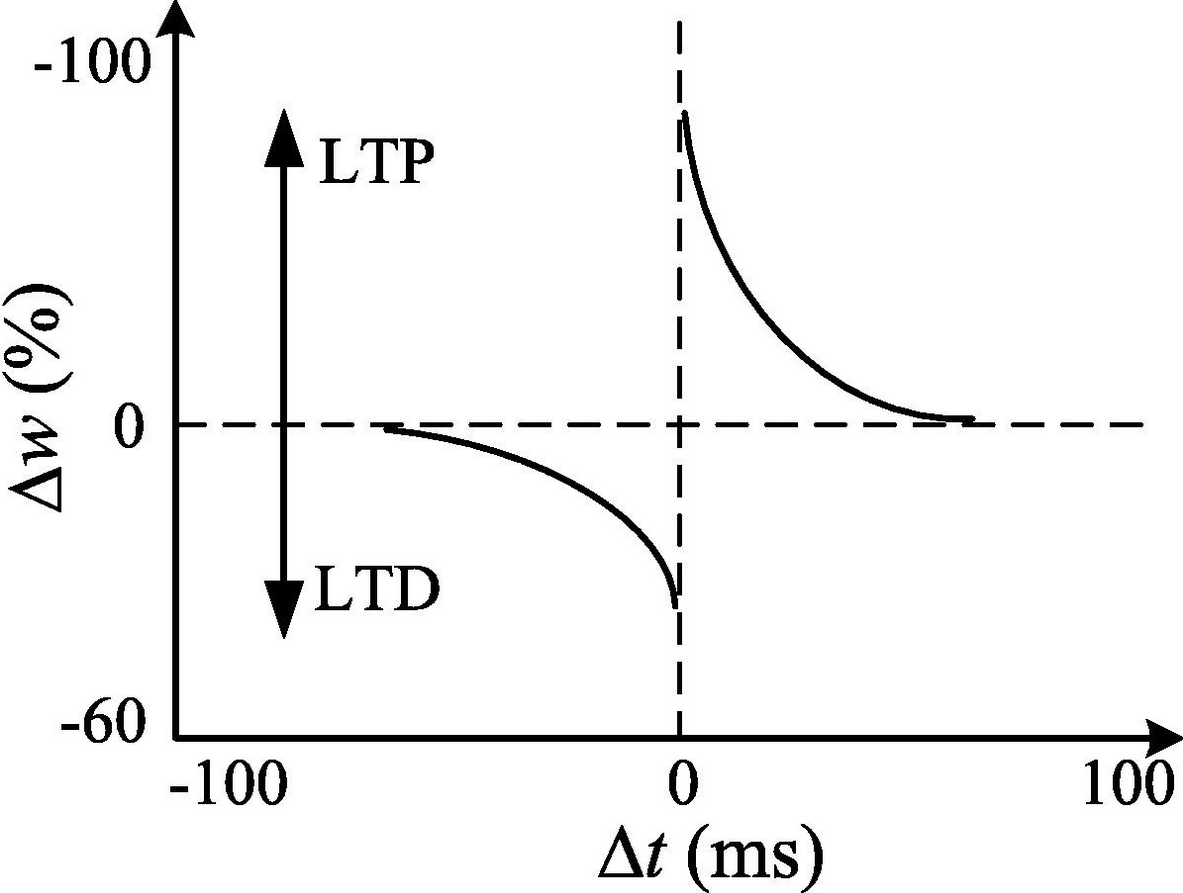
\includegraphics[scale = 0.15]{stdp}
	\caption{Graphical representation of STDP learning rule. Weight change depending on the time between pre- and postsynaptic activation. Negative time is the time between the postsynaptic neuron firing before the presynaptic. Graphic taken from \cite{yi_learning_2023}.}
	\label{fig:stdp}
\end{figure}
In addition to the Hebbian rule, there is also the anti-Hebbian rule that is reverses the aforementioned behaviour. This means that regular firing of pre- and postsynaptic neurons is discouraged and more irregular and distributed spiking is favoured. This can be understood as mirroring \cref{fig:stdp} along the x-axis.\\

These rules are based in biology and satisfy the restrictions found in nature. Many learning rules adapted from \acp{ANN} lack these properties e.g. locality. Locality demands that the basis of learning is restricted to having only the information of the direct pre- and postsynaptic neuron available. This already rules out most backpropagation algorithms as the come derive the derivative with respect to a global cost function.\\

Of course there many variations and extensions have been proposed, e.g. \ac{SRDP}\cite{kempter_hebbian_1999}, which have been summarized in  \cite{yi_learning_2023}.

